%%%
%%% 编译此TeX文件需要完整的ctex宏集(建议使用TeXLive/MikTeX最新版本配置所需宏)以及所有\usepackage[*]{...}
%%% 命令中需要的名称为...的包
%%% 使用XeLaTeX引擎编译
%%%
\documentclass[8pt]{ctexbeamer}

%	Beamer主题
\usetheme{boxes}
%	Beamer颜色主题
\usecolortheme{seahorse}
%	Beamer内置主题
\useinnertheme{rectangles}
%	Beamer外置主题
\useoutertheme[subsection=false,footline=authortitle]{miniframes}
%	Beamer字体主题
\usefonttheme{default}
\usefonttheme[onlymath]{serif}						%	数学字体主题
%	Beamer导航栏
\setbeamertemplate{navigation symbols}[horizontal]	%	设置导航栏为水平
%	Beamer目录
\setbeamertemplate{section in toc}[square]			%	目录章节设置为方块
%	Beamer无序列表模板
\definecolor{SteelBlue}{RGB}{70,130,180}
\setbeamertemplate{itemize item}[square]			%	使用三角符号进行无序列表枚举
\setbeamercolor{itemize item}{fg=SteelBlue}			%	无序列表itemize环境颜色	
%	Beamer标准块环境
\setbeamercolor{block title}{bg=cyan!50, fg=black}		%	标题颜色
\setbeamercolor{block body}{bg=cyan!10}				%	块主体颜色
%	Beamer章节页设置
\AtBeginSection{
	\begin{frame}
		\begin{beamercolorbox}[sep=25pt,center]{part title}
			{\LARGE	\insertsection}
		\end{beamercolorbox}
	\end{frame}
}

%	集成所需宏
\usepackage{enumerate}							%	枚举环境
\usepackage{graphicx}							%	图片插入
\usepackage{subcaption}							%	子图
\usepackage{amsmath,amsthm,amsfonts,amssymb}    %	使用AMS集成包
\usepackage{xcolor}     						%	颜色
\usepackage{hyperref}							%	超链接

%  文本提示框
\usepackage{tcolorbox}
\tcbuselibrary{skins}
\tcbsetforeverylayer{enhanced}
\newtcolorbox[auto counter,number within=section]{notebox}[1]{
    skin=empty,
    top = 0pt,
    bottom = 0pt,
    toprule = 0pt,
    bottomrule = 0pt,
    leftrule = 0pt,
    rightrule = 0pt,
    borderline west={2pt}{0pt}{#1},
}

% 注释结论
\newenvironment{remark}
{
	\begin{notebox}{orange}
}
{
	\end{notebox}
}

% 引用结论
\renewenvironment{quote}
{
	\begin{notebox}{gray}
}
{
	\end{notebox}
}


\title{华为第一届领航杯应用数学大赛}
\subtitle{低功耗自适应FIR滤波硬件算法}
\date{2023.9.20}
\author{柴昊、李明昊、王熙元}
\institute{复旦大学\\
	南京大学}

%\logo[options]{logo path}	添加LOGO

\begin{document}

% Title page 
\begin{frame}[plain, noframenumbering]
	\titlepage
\end{frame}

\begin{frame}[plain]
	\begin{beamercolorbox}[sep=12pt,center]{part title}
		{\Large	\contentsname}		
	\end{beamercolorbox}
    \tableofcontents
\end{frame}

\section{理论回顾}


\begin{frame}{快速 Fourier 变换(FFT) 处理器算法}{一种浮点FFT流处理器:基于冗余计算和折叠架构的浮点运算蝶形阵列}
	\begin{quote}
		Cooley 和 Tukey 是 Princeton 的两位数学家和计算机科学家,他们首先设计出离散
		傅立叶变换算法 (Discrete Fourier Transformation/ Fast Fourier Transformation, 
		DFT/FFT)。时间复杂度可以达到 $\mathrm{O}(n \ln n)$。
		此方式适用于 $n = 2^m$。
		
		对于 $n \not= 2^m$ 的多项式乘法或卷积,总可以通过引入先导零/占位的方式约化到 $n = 2^m$ 的情形,
		由于 $k$
		和 $2k$ 之间必然有一个 $2$ 的次幂,理论上快速傅立叶变换的时间复杂度不会超过 $\mathrm{O}(2n \ln n)$。
		另外 Cooley-Tukey
		的变形中会处理 $N_1 N_2$ 阶数 FFT,通常分解为 $N_1$ 个 $N_2$ 阶 FFT 处理 (N1 $\ll$ N2)。
	\end{quote}


	\begin{figure}[h!]
		\centering
		\begin{subfigure}[b]{0.4\textwidth}
			\begin{center}
				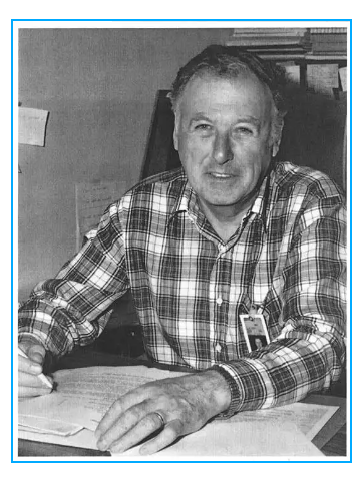
\includegraphics[scale=0.36]{figure/JamesCooley.png}
			\end{center}
			\caption{James Cooley}
		\end{subfigure}
		\hfill
		\centering
		\begin{subfigure}[b]{0.4\textwidth}
			\begin{center}
				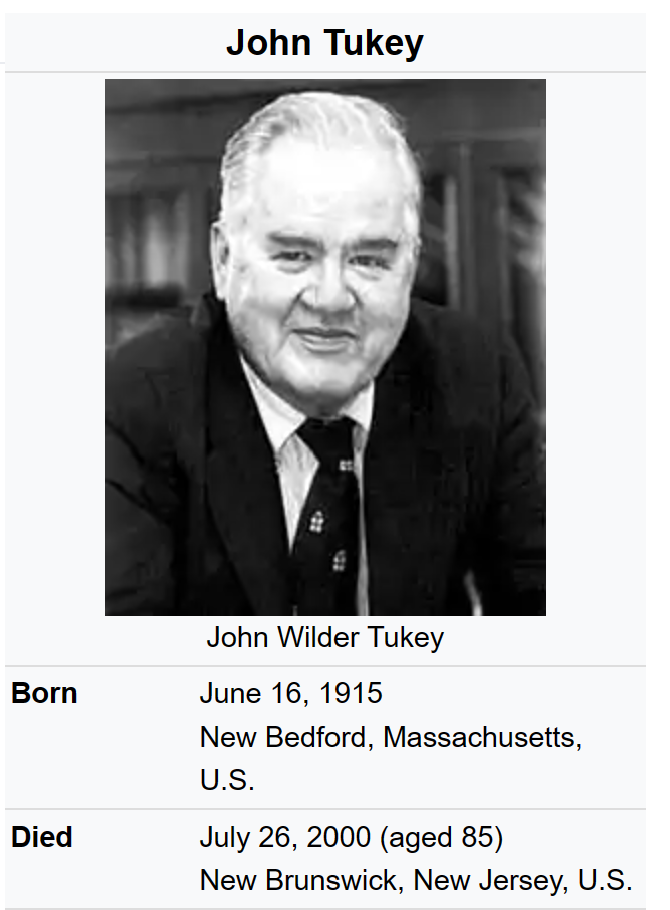
\includegraphics[scale=0.2]{figure/JohnTukey.png}
			\end{center}
			\caption{John Tukey}
		\end{subfigure}
		\caption{发明第一个 FFT 算法的数学家及计算科学家}
		\label{fig:Cooley-Tukey}
	\end{figure}


\end{frame}

\begin{frame}{冗余计算加速算法}{基四最小冗余混合加法(mrHY4A)}
	\begin{block}{算法架构简介}
		本项目选用了基四最小冗余(Minimal Redundant Radix-4,mr4)方案,
		对于任意一个 $2n$ 二进制位的整
		数 $X \in \mathbb{Z}$,其 mr4 冗余表达式为:
		\[
			X = \sum_{i=0}^{i=n-1} [x_i] 4^i,\quad [x_i] \in \left\{-2,-1,0,1,2\right\} 
		\]
		而数位 $[x_i] $ 用三个 bit $(x_i^{-2} , x_i^{+}, x_i^{++}) \in \left\{0,1\right\}^{3}$ 表示为
		\[
			[x_i] = -2 x_i^{-2}	+ x_i^+ + x_i^{++}
		\]
	\end{block}
	
	其优势至少体现在以下三点。

	\begin{quote}
		\begin{itemize}
			\item 冗余示数法具有多映射的特点实现无\textbf{进位传播}的冗余加法
			\item 大端和小端先入结构的硬件优势
			\item mr4 冗余表示不需要符号位
		\end{itemize}
	\end{quote}
\end{frame}

\begin{frame}{与无优化算法对比}
	\begin{center}
		\begin{figure}
			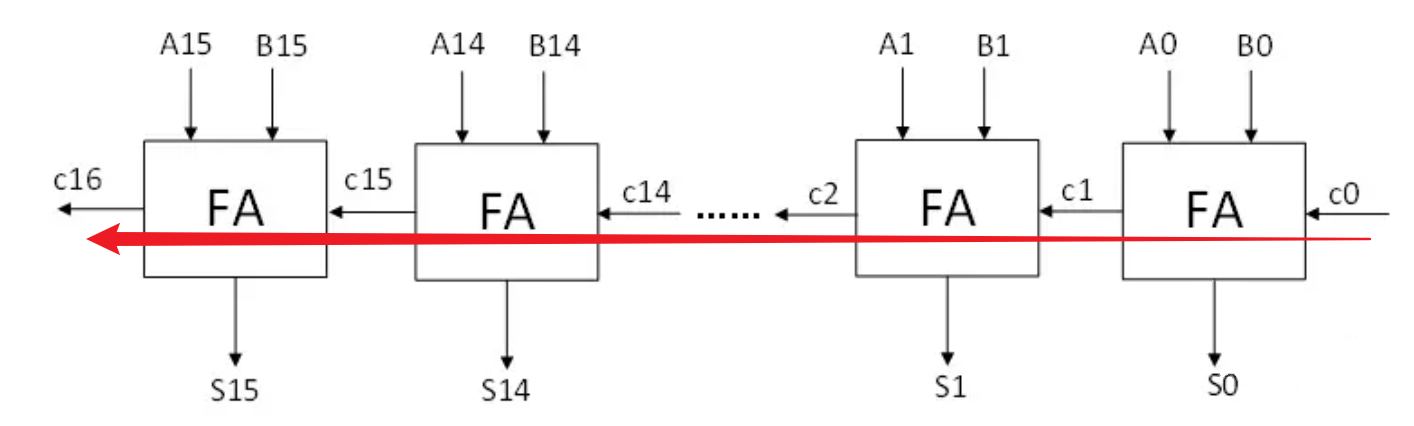
\includegraphics[width=0.8\textwidth]{figure/NonRedundant.png}
			\caption{非冗余计算形式}
			\label{fig:NonR}
		\end{figure}
		\begin{figure}
			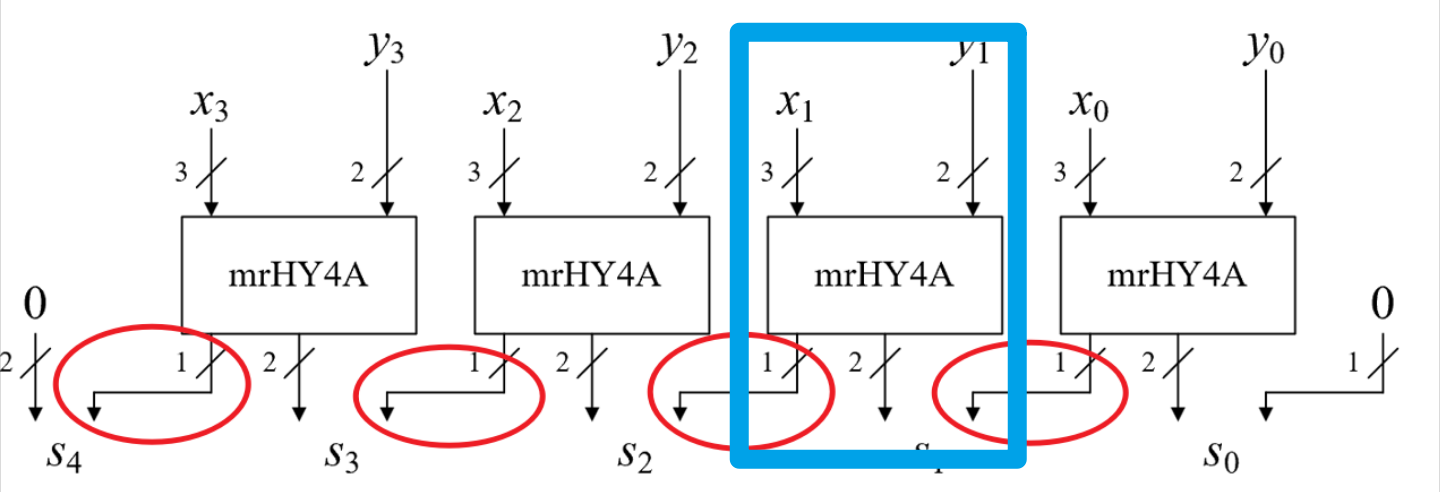
\includegraphics[width=0.8\textwidth]{figure/Redundant.png}
			\caption{冗余4计算形式}
			\label{fig:R}
		\end{figure}
	\end{center}
\end{frame}

\section{算法实现与创新}

\begin{frame}{优化思路一}{采用各层同形的FFT拓扑结构优化绕线}

	\begin{center}
		\begin{figure}
			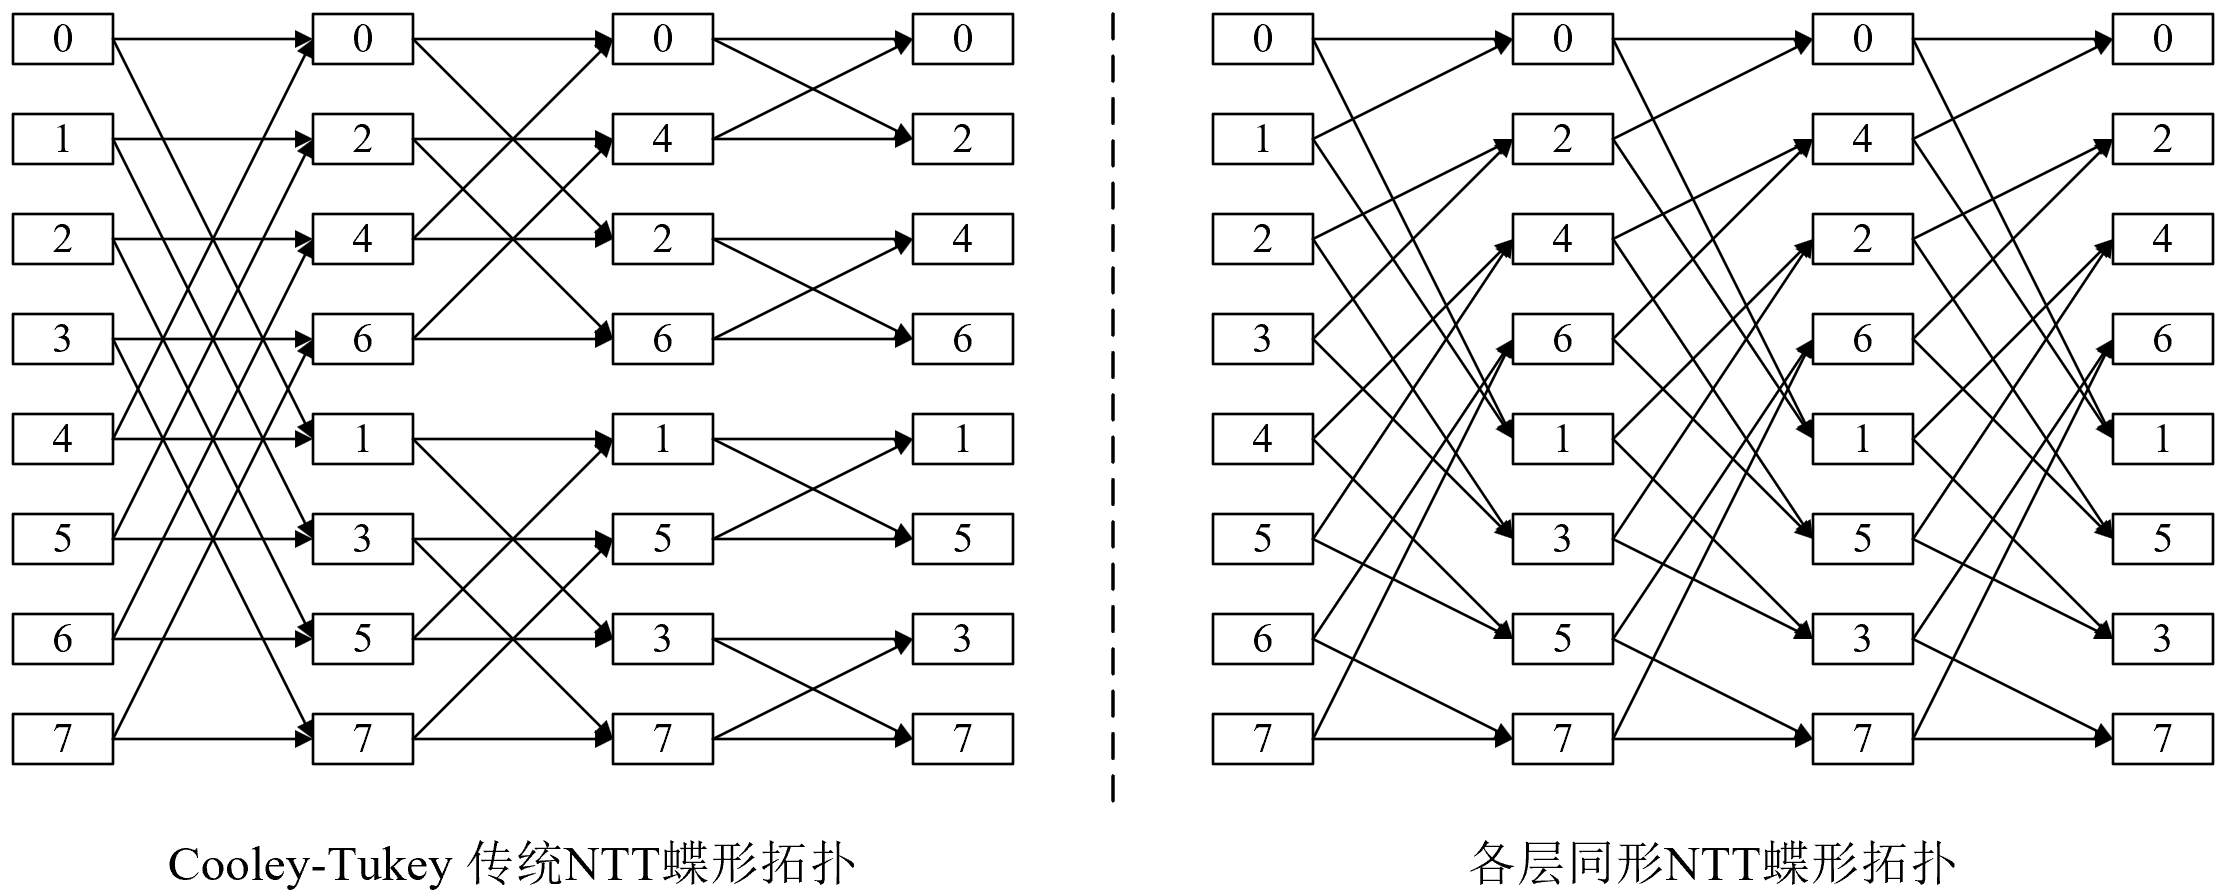
\includegraphics[width=0.9\textwidth]{figure/Figure1.NTT_Topology.png}
			\caption{不同绕线方式比较}
			\label{fig:FFTComparison}
		\end{figure}
	\end{center}

	并行FFT设计中,传统的Cooley-Tukey蝶形拓扑的各层绕线复杂度不同。
	\begin{quote}
		具体记各层布线复杂度 $O_1 > O_2 >\cdots > O_{\log_2 N}$ (一般后层布线更迅速)。则硬件实现拓扑复杂度是
		关于 $O_1,..,O_{\log_2 N}$ 的带权函数。
	\end{quote}
\end{frame}

\begin{frame}{优化思路二}{通过蝶形运算Folding架构}
	\begin{columns}
		% Column 1
		\begin{column}{0.5\textwidth}
			\begin{center}
				\begin{figure}
					\centering
					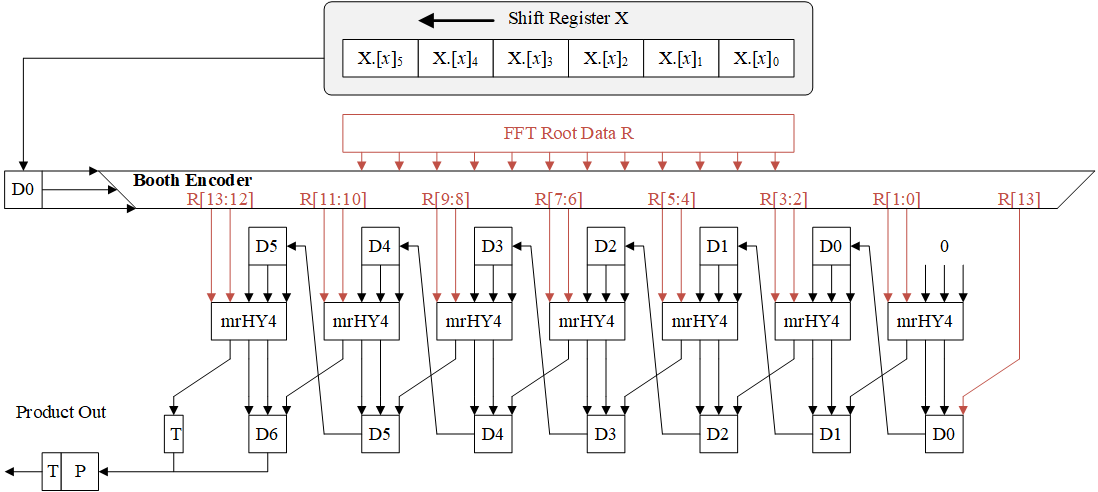
\includegraphics[width=0.9\textwidth]{figure/Figure2.Multiplier.png}
					\caption{mr4HY串行乘法器}
					\label{fig:Multiplier}
				\end{figure}
			\end{center}
			\begin{quote}
				好处:降低绕线复杂度;降低浮点运算复杂度;减小并行压力。
			\end{quote}
		\end{column}
		% Column 2    
		\begin{column}{0.5\textwidth}
			\begin{center}
				\begin{figure}
					\centering
					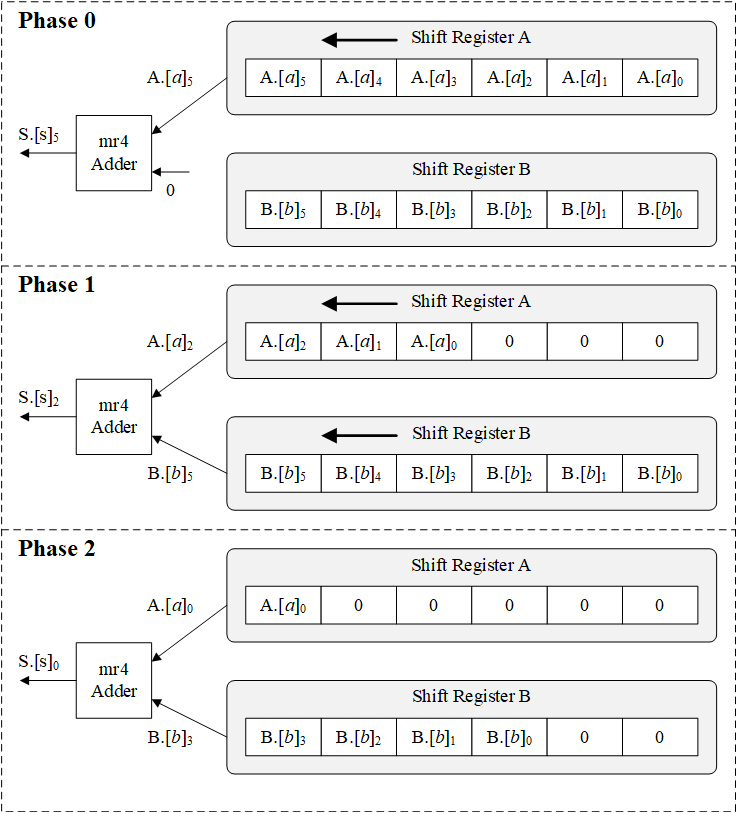
\includegraphics[width=0.9\textwidth]{figure/Figure3.Float_Adder.png}
					\caption{mr4HY串行浮点加法器}
					\label{fig:Adder}
				\end{figure}
			\end{center}
		\end{column}
	\end{columns}

\end{frame}

\begin{frame}{流处理器工作管道}
	\begin{center}
		\begin{figure}
			\centering
			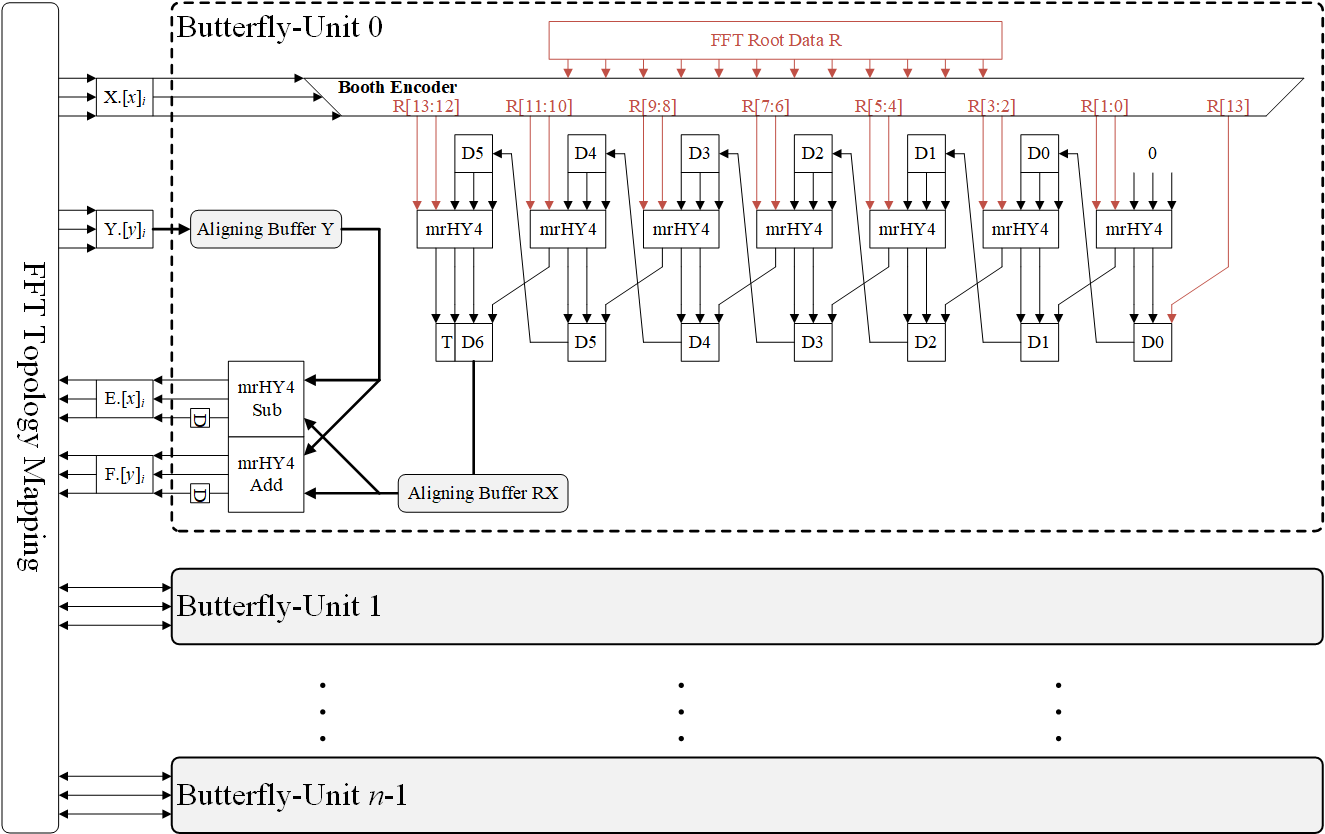
\includegraphics[width=0.65\textwidth]{figure/Figure4.Float_BU.png}
			\caption{蝶形运算阵列}
			\label{fig:Float_BU}
		\end{figure}

		\begin{enumerate}[a)]
			\item {\scriptsize 第一级流水线为冗余乘法:FFT上一级蝶形运算输出,经过Mapping拓扑映射单元送往当前蝶形运算输入端,
			随输入数据串入,乘法执行结束,与此同时,乘法器输出逐个数位地输入Aligning Buffer中,
			便于后续冗余加减法操作; }
			\item {\scriptsize 第二级流水线为冗余浮点加减法:从Aligning Buffer先后输出数据被加减归约,
			其输出至Mapping单元,以便送达FFT下一级蝶形运算对应蝶形结输入端。}
		\end{enumerate}
	\end{center}
\end{frame}

\begin{frame}{技术优势}
	本方案使用\textbf{折叠展开架构},本
	质上是在 \textbf{蝶形运算并行度} 和 \textbf{\textbf{FFT} 每级内蝶形并行个数}之间做权衡,
	通过内部折叠蝶形,外部展开计算阵列,完成拓扑结构的化简与计算流程的化简。

	\begin{block}{降低绕线复杂度的方法}
		\begin{enumerate}
			\item 采用各层同形拓扑
			\item 采用 Digital Serial 处理结构
		\end{enumerate}
	\end{block}

	\begin{block}{其他设计收益}
		\begin{enumerate}
			\item 冗余串行算法降低浮点运算复杂度
			\item 大端输入减小系统延迟
			\item 流处理结构的控制逻辑非常简单
		\end{enumerate}
	\end{block}

	进一步的优化思路:可以利用Twiddle factor常数乘法的特点,对串行乘法器做进一步简化。

\end{frame}

\begin{frame}{性能比较}{基于  Xilinx Artix-7 仿真系统数据}

	\begin{center}
		\begin{figure}
			\centering
			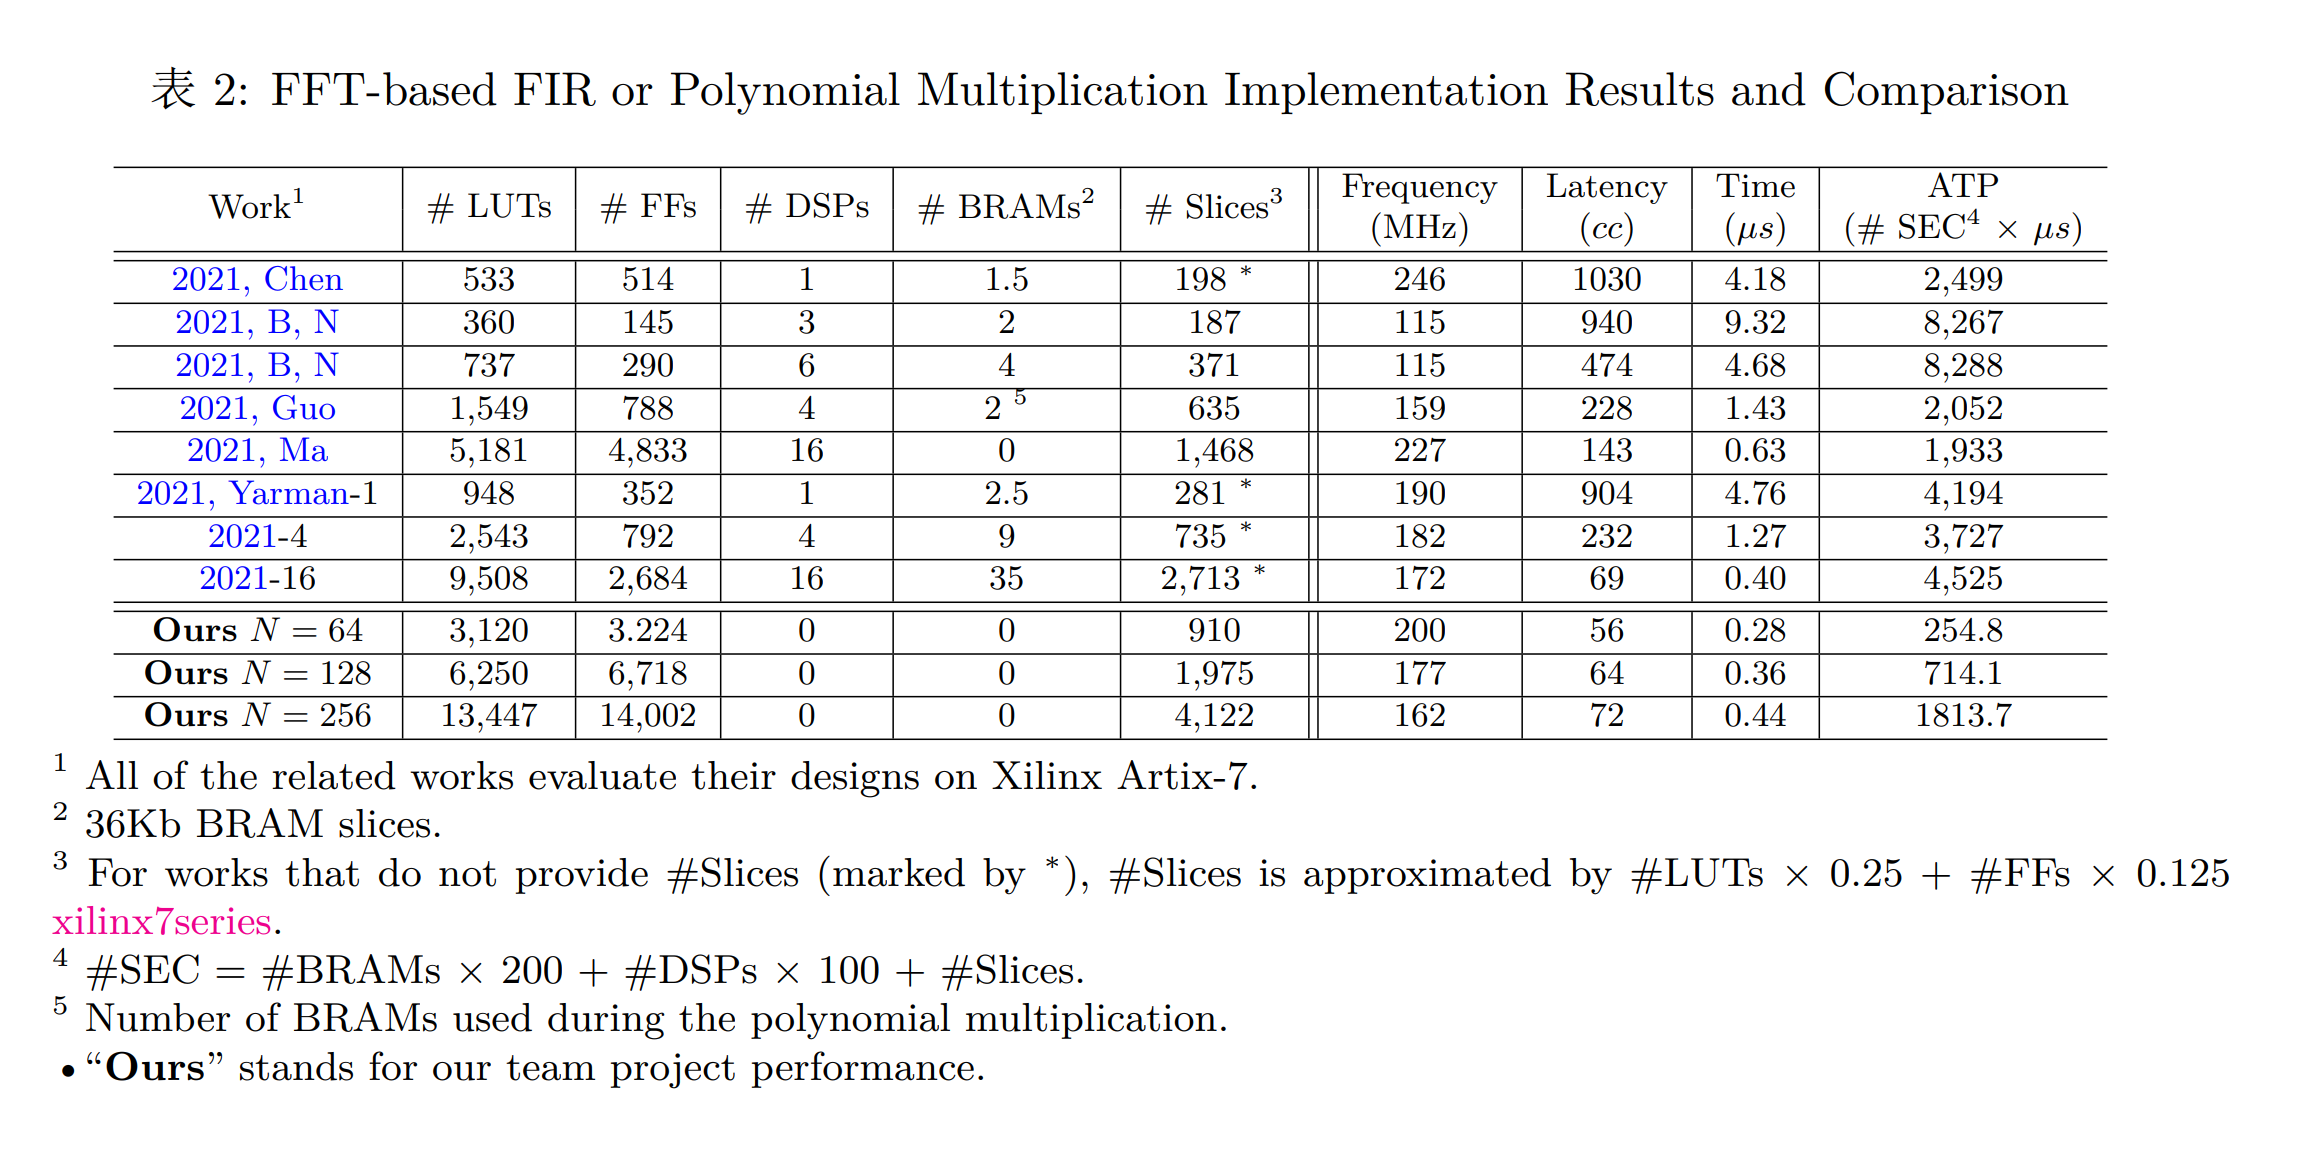
\includegraphics[width=0.99\textwidth]{figure/Comparison.png}
			\caption{本团队工作和其他已知算法的性能比较}
			\label{fig:Comparison}
		\end{figure}
	\end{center}
\end{frame}

\section{后续计划}

\begin{frame}{基于量化感知进行信号预测和自适应处理}{通过 OpenNN C++ 神经网络框架}
	\begin{quote}
		使用 OpenNN 神经网络框架搭建量化感知算法
	\end{quote}
	\begin{quote}
		回顾上部分的 Twiddle Factor 近似技术加速硬件运算
		\begin{center}
			\begin{figure}
				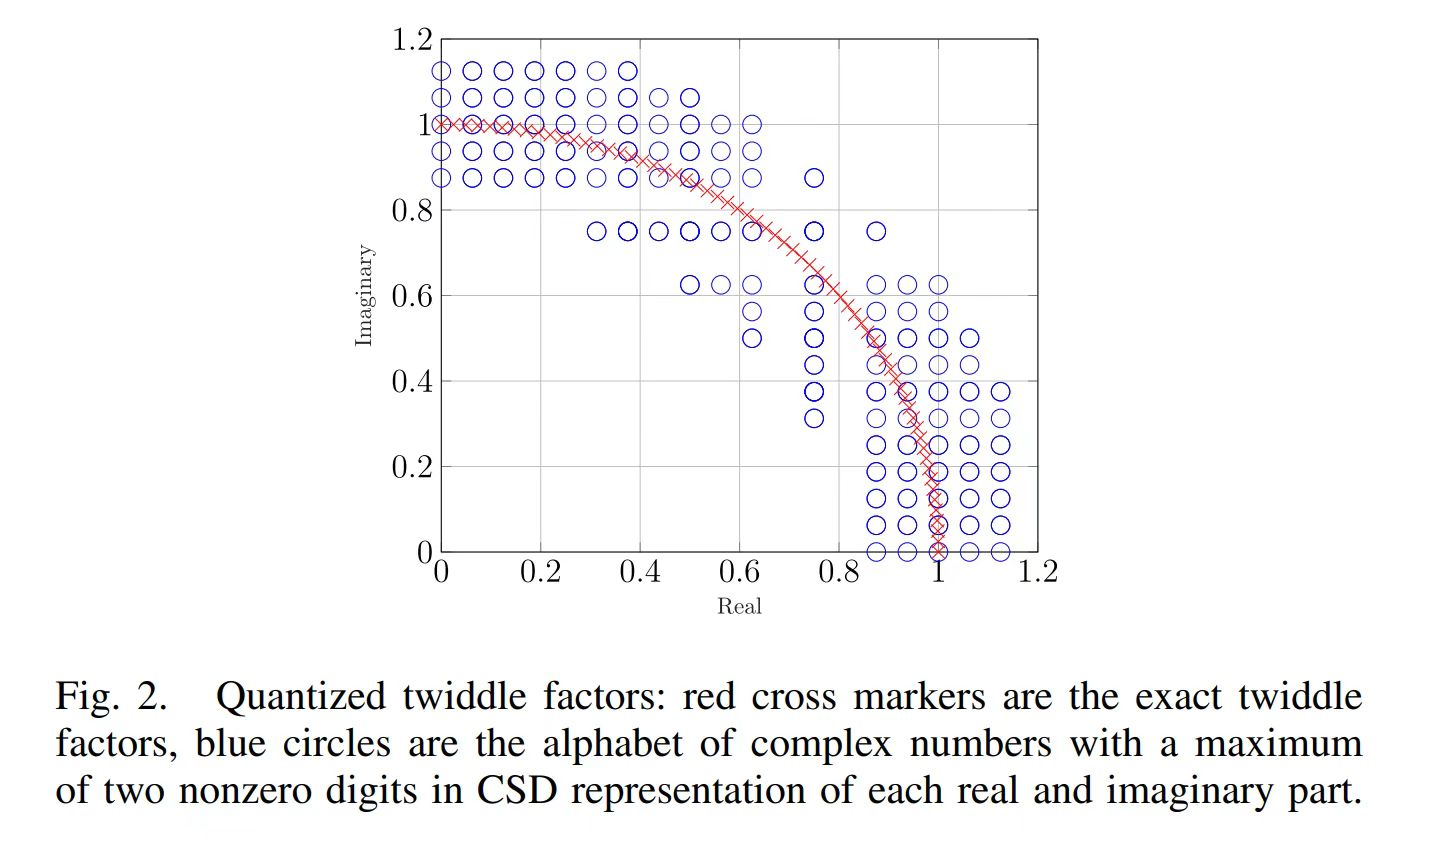
\includegraphics[width=0.8\textwidth]{figure/TwiddleFactor.png}
				\caption{近似 FFT 与 Twiddle Factor}
				\label{fig:Twiddle Factor}
			\end{figure}
		\end{center}
	\end{quote}
\end{frame}

\begin{frame}{基于此高效 FFT 流处理器的降噪/变频算法}{基于不同应用场景}
	\begin{quote}
		\begin{itemize}
			\item 射频波段的频率俘获/提纯硬件算法:\\
				{\fontsize{5pt}{2pt}\selectfont 具体理论来自数字信号处理/小波分析}
			\item 全频带的自适应信号预测:\\
				{\fontsize{5pt}{2pt}\selectfont 
				将主要基于此次竞赛实现的流信号处理器,使用贝叶斯网络或智能Pid控制策略设计算法}
			\item 声学波段的主动降噪算法:\\
				{\fontsize{5pt}{2pt}\selectfont 
				希望可以开发出能使用在蓝牙耳机/通话系统等硬件的降噪功能模块上}
		\end{itemize}
	\end{quote}

	最后,此项工作也有更深层次的理论意义,即开发更快的浮点乘法和 Fourier 变换运算器。这在图像处理,数值计算
	等领域都是重要的。
\end{frame}

\section{致谢}

\begin{frame}
	\begin{center}
		\Huge\textbf{报告结束\, 感谢聆听}
	\end{center}
\end{frame}

\end{document}


% %	命令简化
% \newcommand{\Z}{\mathbb{Z}}
% \newcommand{\E}{\mathbb{E}}
% \newcommand{\Prob}{\mathbb{P}}
% \newcommand{\Var}{\mathbf{Var}}
% \newcommand{\R}{\mathbb{R}}
% % 	数学符号Stirling数
% \newcommand{\genstirlingI}[3]{%
%   \genfrac{[}{]}{0pt}{#1}{#2}{#3}%
% }
% \newcommand{\genstirlingII}[3]{%
%   \genfrac{\{}{\}}{0pt}{#1}{#2}{#3}%
% }													%	第一类第二类Stirling数
% \newcommand{\stirlingI}[2]{\genstirlingI{}{#1}{#2}}
% \newcommand{\dstirlingI}[2]{\genstirlingI{0}{#1}{#2}}
% \newcommand{\tstirlingI}[2]{\genstirlingI{1}{#1}{#2}}
% \newcommand{\stirlingII}[2]{\genstirlingII{}{#1}{#2}}
% \newcommand{\dstirlingII}[2]{\genstirlingII{0}{#1}{#2}}
% \newcommand{\tstirlingII}[2]{\genstirlingII{1}{#1}{#2}}
%	Beamer章节页
% \definecolor{C1}{RGB}{0,62,128}
% \definecolor{C2}{RGB}{0,159,227}
% \definecolor{GRAY1}{RGB}{245,245,245}
% \setbeamercolor{titlepage}{fg=GRAY1,bg=C1}		%	颜色使用
% \setbeamertemplate{section page}
% {
% 	\nointerlineskip
% 	\begin{beamercolorbox}[dp=2.3ex, sep=2ex, wd=\paperwidth, ht=\paperheight]{titlepage}
% 		\vbox to 35ex{
% 			\hspace{0.16\linewidth}
% 			\begin{minipage}[c]{0.6\linewidth}
% 				{\Large \bfseries \insertsection}

% 				\begin{tikzpicture}
% 					\draw[line width=0.5pt, color=C2] (0,0) -- (\linewidth,0);
% 				\end{tikzpicture}
% 			\end{minipage}
% 		}
% 	\end{beamercolorbox}
% }
%

%	补充所需宏
%\usepackage{mdframed}       					%	用mdframe设置定理样式
%\usepackage{zref}								%	引用格式翻新
%\usepackage{tikz-cd}							%	tikz绘图
%\usepackage{verbatim}							%	代码输入等